\documentclass[11pt]{article}
\usepackage[margin=1in]{geometry}
\usepackage{amsmath,amssymb,amsthm,mathtools}
\usepackage{booktabs,graphicx,hyperref}
\hypersetup{
  colorlinks=true,
  allcolors=blue,
  pdftitle={Certified coexistence of symmetry-reduced local maximizers for enstrophy production in a periodic 3D Navier--Stokes Fourier class},
  pdfauthor={Avighna Wuthoo},
  pdfsubject={Finite-dimensional computer-assisted variational theorem},
  pdfkeywords={Navier--Stokes, enstrophy production, computer-assisted proof, interval arithmetic, Fourier--Galerkin}
}

\newtheorem{theorem}{Theorem}[section]
\newtheorem{proposition}[theorem]{Proposition}
\newtheorem{remark}[theorem]{Remark}
\newcommand{\T}{\mathbb{T}}
\newcommand{\R}{\mathbb{R}}
\newcommand{\E}{\mathcal{E}}
\newcommand{\rate}{\mathcal{R}}

\title{Certified coexistence of symmetry-reduced local maximizers\\
in a periodic 3D Navier--Stokes Fourier class}
\author{Avighna Wuthoo}
\date{}

\begin{document}
\maketitle

\begin{abstract}
We study the classical fixed-enstrophy variational problem for instantaneous
enstrophy production in periodic three-dimensional Navier--Stokes flow, within
a prescribed 16-pair Fourier class with 64 real divergence-free coordinates.
We give two exact symmetry reductions. The first is a six-amplitude fixed
space on which a Sturm and interval-arithmetic calculation proves the global
maximum of the static rate. Its high-parameter branch is global within that
symmetry class above an explicit threshold. The second is a two-amplitude
fixed space with a closed-form stationary branch and a closed optimized-rate
formula. Symbolic algebra verifies that it is a full 64-coordinate KKT branch
for every positive enstrophy and viscosity. A rational interval cover with
separate 256- and 512-bit Arb calculations certifies this branch as a strict
full-space local maximum modulo translations for every such parameter pair.
The high-parameter six-amplitude branch is independently certified as a
strict full-space local maximum throughout its entire existence range.
At the inviscid endpoint, the explicit six-amplitude limiting field is also
certified as a strict full-space local maximum of stretching, modulo
translations; together with the competing branch it gives two distinct exact
full-space local maxima with an explicit value gap.
An exact rational sum-of-squares certificate also controls the $(1,1,2)$
shell component of the stretching cubic, while leaving cross-component
alignment open.
At 10,000 it exceeds the six-amplitude rate. The two symmetry
branches cross exactly once at an interval-certified dimensionless parameter
value near 27,993. All
statements are finite
dimensional; none addresses global regularity or singularity formation for the
Navier--Stokes PDE.
\end{abstract}

\paragraph{Key words.} Navier--Stokes equations; enstrophy production;
computer-assisted proof; interval arithmetic; Fourier--Galerkin methods.
\paragraph{MSC codes.} 76D05, 65G40.

\section{Introduction}
For a periodic incompressible velocity field, the instantaneous production of
enstrophy is a natural diagnostic for extreme three-dimensional flows.  The
fixed-enstrophy variational problem was studied numerically by Lu and Doering
\cite{LuDoering2008} and by Ayala and Protas \cite{AyalaProtas2017}; those
works established important extreme-flow branches but did not give an exact
finite-enstrophy, computer-assisted classification of a prescribed Fourier
class.  We give such a classification for two symmetry-fixed subspaces of a
64-dimensional Fourier polynomial.

The novelty claimed here is deliberately narrow: exact Fourier reductions,
exact algebraic branch formulas, and computer-assisted local maximality in a
specified finite class.  This differs from numerical optimization of the
unrestricted PDE problem \cite{LuDoering2008,AyalaProtas2017,KangYunProtas2020}
and from Fourier-restricted model equations with a modified projection
\cite{Miller2025}, as well as recent orbit-level Galerkin analyses
\cite{Kiriukhin2026,KiriukhinTransfer2026}. The
finite-dimensional result should not be read as a statement about Navier--
Stokes regularity.

\section{Static Fourier variational problem}
On $\T^3=[0,2\pi)^3$, let
\[
 \partial_t u+(u\cdot\nabla)u+\nabla p=\nu\Delta u,\qquad \nabla\cdot u=0.
\]
With $\omega=\nabla\times u$ and $S=(\nabla u+\nabla u^T)/2$, set
\[
 \E=\frac12\langle|\omega|^2\rangle,\quad
 P=\frac12\langle|\nabla\omega|^2\rangle,\quad
 A=\langle\omega\cdot S\omega\rangle,\quad
 \rate=A-2\nu P.
\]
We restrict $u$ to the canonical divergence-free polarization basis on the 16
independent pairs $0<|k|^2\leq4$, yielding $x\in\R^{64}$.  Our static problem
is $\max\{\rate(x):\E(x)=E_0\}$.

\subsection{Exact Fourier and symmetry conventions}
For reproducibility, we state the finite-dimensional model precisely. Let
$\mathcal K$ contain the lexicographically positive representative of every
pair $\{k,-k\}$ with $0<|k|^2\leq4$. Thus $|\mathcal K|=16$. For each
$k\in\mathcal K$, choose the coordinate vector $e_j$ whose corresponding
entry of $k$ has least absolute value (breaking ties by $j$), and set
\[
 p_1(k)=k\times e_j,\qquad p_2(k)=k\times p_1(k).
\]
The real and imaginary coefficients of $p_1(k)$ and $p_2(k)$ give the four
real coordinates for the pair, while $\widehat u(-k)=\overline{\widehat
u(k)}$. These integer polarizations fix the 64-coordinate convention used in
every theorem and archive.

All convolution, Leray projection, and inner products in the certificates are
performed over $\mathbb Q(\mathrm{i})$. In particular, if
$B(v,w)=-\mathbb P[(v\cdot\nabla)w]$, then the cubic term is evaluated as
$A=\langle\nabla\times u,\nabla\times B(u,u)\rangle$ by exact finite
Fourier sums. There is no floating-point identification of the displayed
reduced polynomials.

For a signed-coordinate orthogonal matrix $Q$ and $m\in\mathbb Z^3$, write
\[
 (g_{Q,m}u)(x)=Q u\!\left(Q^T\!\left(x-\frac{\pi m}{2}\right)\right).
\]
On Fourier coefficients this is
\[
 \widehat{g_{Q,m}u}(k)=Q\widehat u(Q^Tk)
 \exp\!\left(-\mathrm{i}\,Q^Tk\cdot\frac{\pi m}{2}\right).
\]
This action preserves $\E$, $P$, and $A$. We form common fixed spaces by exact
rational row reduction of $g_{Q,m}-I$ in the above 64 coordinates.

\subsection{An exact shellwise SOS bound}
Write $E_j$ for the enstrophy carried by the $|k|^2=j$ shell, and let
$A_{112},A_{123},A_{224},A_{334}$ denote the four parts of the exact stretching
cubic, indexed by their squared-shell patterns.
The following finite-class
estimate is a useful check on the exact cubic algebra.
\begin{proposition}[A rational SOS shell bound]\label{prop:shell112}
In the canonical 16-pair Fourier class,
\begin{align*}
 A_{112}^2\leq \frac43 E_1^2E_2,
 &\qquad |A_{112}|\leq \frac{2}{\sqrt3}E_1\sqrt{E_2},\\
 A_{123}^2\leq16E_1E_2E_3,
 &\qquad A_{224}^2\leq E_2^2E_4,\\
 |A_{224}|\leq E_2\sqrt{E_4},
 &\qquad A_{334}^2\leq\frac2{27}E_3^2E_4.
\end{align*}
\end{proposition}
\begin{proof}[Exact certificate]
For each pattern, write the cubic as $\sum_j M_j(y)z_j$ in the coordinates of
the repeated and linear shells. Weighted Cauchy reduces the claim to a quartic
in $y$. The $(1,1,2)$ quartic is represented on 78 degree-two monomials by a
rational Gram matrix with 40 positive Schur pivots and a 38-dimensional zero
remainder. The $(2,2,4)$ quartic has a separate rational Gram matrix on 300
degree-two monomials, with 106 positive pivots and a 194-dimensional zero
remainder. In both cases exact coefficient expansion agrees with the Fourier
cubic, hence $G\succeq0$ over $\mathbb Q$. The other two patterns are checked
by separate exact Gram identities: a 288-by-288 positive-definite bilinear
Gram matrix for $(1,2,3)$, and a sparse rank-three 136-by-136 Gram matrix for
$(3,3,4)$. These are bounds for individual triad components only: they neither
prove sharp constants nor bound the full stretching cubic.
\end{proof}

\subsection{Certified local statements}
For a phase slice, the constrained stationarity equations consist of the 64
rate equations, the enstrophy constraint, and three translation phase
conditions. The resulting 68-dimensional polynomial system is evaluated with
outward-rounded Arb balls. Strict inclusion of its Krawczyk image in a box
proves a unique zero in that box \cite{Krawczyk1969}. An exact-dyadic
congruence followed by interval Gershgorin bounds gives the bordered inertia.
The reported inertia $(4,64,0)$ proves nondegeneracy and the strict constrained
local maximum modulo the three translations. This is a local statement in the
stated Fourier class only.

\section{Six-amplitude branch}
Three combined signed-coordinate and quarter-period translation symmetries
have a six-dimensional common fixed space.  Exact rational row reduction
identifies coordinates $(a,b,c,d,e,f)$ in which
\begin{align}
 A&=64acd+32aef-64bdf,\label{eq:sixA}\\
 \E&=2a^2+32b^2+48c^2+8d^2+48e^2+4f^2,\label{eq:sixE}\\
 P&=2a^2+128b^2+144c^2+16d^2+144e^2+8f^2.\label{eq:sixP}
\end{align}

\begin{theorem}[Certified ansatz globality]\label{thm:six}
At $\nu=10^{-2}$ and $\E=100$, the constrained maximum of $\rate$ in the
six-amplitude fixed space is unique after the finite sign gauge and equals
\[449.718337230445715677500657\ldots.\]
The corresponding full 64-coordinate point is a strict local maximum modulo
translations.
\end{theorem}

The proof combines exact face exhaustion, Sturm isolation of the interior
multiplier root, and separate 256/512-bit Arb comparisons.  Symmetric
criticality promotes restricted stationarity to full-space stationarity
\cite{Palais1979}; a 68-variable Krawczyk inclusion and certified bordered
inertia $(4,64,0)$ give the local statement.  The interval inclusion is used
in its usual existence-and-uniqueness role \cite{Krawczyk1969}.

Writing $\eta=\E/\nu^2$ and $\mu=\lambda/\nu$, the high-$\eta$ interior
branch satisfies
\begin{equation}\label{eq:quartic}
69\mu^4+1696\mu^3+(14936-32\eta)\mu^2
+(54656-512\eta)\mu+(68368-2048\eta)=0.
\end{equation}
Descartes' rule and an exact sign bound at $\sqrt{28}$ imply a unique
admissible positive root for $\eta>1867/4$.  Positive-coefficient face
resultants prevent crossing of the interior and face branches, hence the
interior branch is global inside this symmetry class throughout that range.

\begin{theorem}[High-parameter six-amplitude branch]\label{thm:highsix}
For every $\eta>1867/4$, the quartic \eqref{eq:quartic} has one admissible
positive interior root. The associated stationary point is the global
maximizer of $\rate$ within the six-amplitude fixed space, after the finite
sign gauge. This theorem makes no full 64-coordinate global assertion.
\end{theorem}

\begin{theorem}[Uniform full-space stability of the high-$\eta$ six branch]
\label{thm:uniformsix}
For every $\eta>1867/4$, the branch in Theorem~\ref{thm:highsix} is a
strict local maximizer of $\rate$ subject to fixed $\E$, modulo translations,
in the complete 64-real-coordinate Fourier class. This is not a full-space
global-maximality statement.
\end{theorem}

\begin{proof}[Certificate outline]
Put $r=\mu^{-1}=s/10$. At $\eta=1867/4$, the left side of
\eqref{eq:quartic} at $\mu=10$ equals $-344736$; uniqueness of the positive
root therefore gives $0<s<1$ throughout the physical branch. On the compact
auxiliary cover $0\leq s\leq1$, exact radical branch formulas define the
full bordered Hessian after a fixed quarter-period translation to a regular
three-phase slice. At the midpoint of each of 2,048 rational boxes, Arb
certifies bordered inertia $(4,64,0)$. The Frobenius-norm bound
$\|B(s_0)^{-1}(B(s)-B(s_0))\|_F<1$ on each box gives a nonsingular symmetric
homotopy, hence preserves inertia across the box. Independent 256- and
512-bit covers close. The source-bound record is
{\ttfamily six\_branch\_high\_eta\_uniform.json}.
\end{proof}

\section{A competing two-amplitude branch}
Two different lattice symmetries have a two-dimensional common fixed space.
They are
\[
 (Q_1,m_1)=\left(\operatorname{diag}(-1,1,1),(0,2,0)\right),\qquad
 (Q_2,m_2)=\left(
 \begin{pmatrix}0&-1&0\\0&0&1\\-1&0&0\end{pmatrix},(0,0,0)\right).
\]
Exact row reduction gives fixed-space dimension two; the two displayed
generators themselves, rather than a numerically discovered sparsity pattern,
define the ansatz.
Their exact finite closure has 24 elements and is internally isomorphic to
$A_4\times C_2$: it has a central order-two inversion--translation and an
$A_4$ complement. This group identification is obtained by exact multiplication
of signed-coordinate matrices and quarter-period translations. It is a
structural description of the ansatz symmetry, not a parameter-uniform
stability claim. Its exact action on the 64 real controls has isotypic ranks
$(2,6,24)$ in each of the two central-$C_2$ parity sectors; this decomposition
is included to expose the block structure relevant to local stability, but no
uniform Hessian-sign conclusion is drawn here.
In the canonical basis, three coordinates equal $a$, six equal signed copies
of $b$, and all other coordinates vanish.  Exact convolution gives
\begin{equation}\label{eq:twoformula}
A=24a^2b,\qquad \E=3a^2+48b^2,\qquad P=3a^2+96b^2.
\end{equation}
Recovering the entire restricted quadratic/cubic coefficient table directly
from the full rational 64-mode convolution gives respectively
$(3,0,48)$, $(3,0,96)$, and $(0,24,0,0)$ in the monomial orders
$(a^2,ab,b^2)$ and $(a^3,a^2b,ab^2,b^3)$. Thus \eqref{eq:twoformula} is an
identity of polynomials, not an interpolation through candidate points.
The same exact Fourier calculation gives kinetic energy and helicity
\[
 K=3a^2+24b^2,\qquad H=\langle u\cdot\nabla\times u\rangle=0.
\]
Thus the entire competing symmetry plane is nonhelical; this is a structural
description of this branch, not a general feature of enstrophy extremizers.
Moreover, the $a$ modes lie entirely on the $|k|^2=1$ shell and the $b$ modes
entirely on the $|k|^2=2$ shell. The exact cubic $24a^2b$ is therefore a
specific nonhelical two-shell interaction, rather than a diffuse low-mode
superposition.
Equivalently, the branch has the explicit real-space representative
\begin{equation}\label{eq:physicalbranch}
u_{a,b}(x,y,z)=
\begin{pmatrix}
-2a\cos y-8b\sin y\cos z\\
2a\cos z+8b\cos x\sin z\\
2a\cos x-8b\sin x\cos y
\end{pmatrix}.
\end{equation}
Thus the formula can be checked directly in physical space or from the 18
Fourier coefficients archived by the standalone rational audit.
Eliminating $a$ yields
\[
\rate(b)=8\E b-384b^3-2\nu\E-96\nu b^2,
\quad 0\leq b\leq\sqrt{\E/48}.
\]
Its derivative is strictly decreasing, so the unique sign-gauged maximizer is
\begin{equation}\label{eq:twobranch}
b_*=\frac{\sqrt{\E+\nu^2}-\nu}{12},\qquad
a_*^2=\frac{\E-48b_*^2}{3}.
\end{equation}

Substitution gives a closed formula for the optimized rate on this plane,
\begin{equation}\label{eq:tworate}
 \rate_*(\E,\nu)=\frac{4}{9}\left[(\E+\nu^2)^{3/2}
 -6\E\nu-\nu^3\right].
\end{equation}
For $\E,\nu>0$, it is positive precisely when
\[
 \frac{\E}{\nu^2}>\frac{33+15\sqrt5}{2}.
\]

\begin{theorem}[Exact optimization in the competing plane]
\label{thm:twoplaneglobal}
For every $\E,\nu>0$, after fixing the inessential sign of $a$, the branch
\eqref{eq:twobranch} is the unique global maximizer of $\rate$ subject to
$E(a,b)=\E$ within the two-amplitude symmetry plane.  This is a statement
only about that plane, not the unrestricted Fourier class.
\end{theorem}

\begin{proof}
For a fixed positive $\E$, eliminate $a$ by
$a^2=(\E-48b^2)/3$.  A global maximizer may be sign-gauged to $b\geq0$,
where $0\leq b\leq\sqrt{\E/48}$ and
\[
 \rate(b)=8\E b-384b^3-2\nu\E-96\nu b^2.
\]
Its derivative $8\E-1152b^2-192\nu b$ is strictly decreasing, positive at
zero, and negative at the other endpoint.  Thus it has precisely one interior
zero, which is \eqref{eq:twobranch}; this is the global maximum on the
interval.  For $b\geq0$, the direct comparison
\[
 \rate(b)-\rate(-b)=16b(\E-48b^2)\geq0
\]
handles the opposite half of the constraint circle.
\end{proof}

Direct symbolic reduction of every one of the 64 KKT equations shows that
\eqref{eq:twobranch}, with multiplier $\lambda=8b-2\nu$, is a full-coordinate
KKT branch for all $\E,\nu>0$.  Scaling controls by $\sqrt{\E}$ reduces the
local constrained problem to unit enstrophy with parameter
$\eta=\E/\nu^2$.  On the exact branch, write $s=12b$. Then
\[
a=\frac{\sqrt{3-s^2}}{3},\qquad
\frac{\nu}{\sqrt{\E}}=\frac{1-s^2}{2s},\qquad
\eta=\frac{4s^2}{(1-s^2)^2}.
\]
This last expression maps $0<s<1$ monotonically onto all positive $\eta$.
There is also an exact spectral reduction behind the local calculation.  Let
$D_E$ be the diagonal enstrophy quadratic form and let $H_s$ be the Hessian
of $\rate-\lambda\E$ at this branch, with
$\lambda=5s/3-1/s$.  Since the lattice symmetry group is $A_4\times C_2$,
the generalized operator $D_E^{-1}H_s$ preserves its six real isotypic
sectors.  Exact symbolic Fourier algebra gives, up to a nonzero scalar,
\begin{equation}\label{eq:hessianfactor}
 \chi_s(t)=p_{0,+}p_{2,+}^2p_{3,+}^3
 p_{0,-}p_{2,-}^2t^3(7s^2-3st-9)^3p_{3,-}^3.
\end{equation}
Here $p_{0,+}$ and $p_{0,-}$ have degree two, $p_{2,+}$ and $p_{2,-}$ have
degree three, and $p_{3,+}$ and $p_{3,-}$ have degrees eight and six,
respectively.  For example,
\[
 p_{0,+}=9st^2+(9-3s^2)t+4s^3-12s,
 \qquad
 p_{0,-}=(4s+3t)(s^2-3st-3).
\]
The exact coefficient polynomials for all six factors are archived with the
proof objects.  The multiplicities in \eqref{eq:hessianfactor} are the
symmetry multiplicities, not numerical eigenvalue clustering; the $t^3$
factor is the translation orbit.  This factorization is a structural
identity.  It also gives an exact continuation proof of the signs.  Indeed,
after removal of the displayed $t^3$, the constant term of every factor in
\eqref{eq:hessianfactor} has no root on $0<s<1$ by exact Sturm counts in
$s^2$.  Thus no nontranslation generalized eigenvalue crosses zero.  At the
rational sample $s=1/2$, exact Sturm counts in $t$ give
\[
 (n_+,n_-,n_0)=(1,60,3)
\]
for the full generalized Hessian.  The three zeros are precisely the
translation orbit: its enstrophy-metric Gram determinant is
\[
 \det G_{\rm trans}=\frac{8(3+s^2)^3}{729}>0.
\]
Every nontrivial isotypic sector is $\E$-tangent; in the
remaining trivial-even sector, the $\E$-tangent direction
$w=(16b,-a)$ has exact curvature
\[
 w^T H_s w=\frac{32(s^2-3)(s^2+1)}{3s}<0.
\]
Since $D_E^{-1}H_s$ is similar to a real symmetric matrix, its spectrum is
real and continuous in $s$.  Consequently the constrained Hessian is strictly
negative off translations for every $0<s<1$.  The interval cover below is a
separate Arb cross-check of this symbolic continuation argument.

For $0\leq s\leq47/50$, an exact shell-aware congruence removes the
apparent $1/s$ singularity of the bordered Hessian: the $|k|^2=1$ control
coordinates are scaled by $s^{-1}$, the bordered matrix is multiplied by
$s$, and the resulting entries are simplified algebraically before interval
evaluation. A cover by 188 rational intervals separately certifies inertia $(4+,64-,0)$
of this continuous rescaled form. The direct 238-interval cover of
$9049/10000\leq s\leq1$ certifies the same inertia. The covers overlap,
since $47/50>9049/10000$. Both covers were evaluated separately with
256- and 512-bit Arb arithmetic. For $s>0$, the rescaled form is congruent to
the ordinary bordered Hessian and has the same inertia.

\begin{theorem}[Uniform competing branch]\label{thm:uniformcompeting}
For every $\E,\nu>0$, the branch
\eqref{eq:twobranch} is a strict local maximum of $\rate$, modulo
translations, in the complete 64-real-coordinate Fourier class. This is not
a global-maximality claim.
\end{theorem}

At $(\nu,\E)=(1/10,100)$, the certified rate is
$417.844001666639\ldots$, exceeding the six-amplitude rate
$411.566601974923\ldots$ at the same $\eta=10^4$.

\begin{theorem}[Competing full-space local branch]\label{thm:competing}
At $(\nu,\E)=(1/10,100)$, the branch \eqref{eq:twobranch} is a strict local
maximum of $\rate$ modulo translations in the complete 64-real-coordinate
Fourier class. Its rate is strictly greater than that of the six-amplitude
branch at the same parameter. It is not asserted to be a global maximum of
the 64-coordinate problem.
\end{theorem}

\begin{theorem}[Exact symmetry-branch switch]\label{thm:switch}
On the high-$\eta$ branch in \eqref{eq:quartic}, the rates of the two symmetry
branches cross exactly once, at
\[\eta_\times=27992.671985287174015090\ldots.\]
The two-amplitude rate is larger for $1867/4<\eta<\eta_\times$, and the
six-amplitude rate is larger for $\eta>\eta_\times$.
\end{theorem}

\begin{proposition}[Exact high-parameter efficiency]\label{prop:efficiency}
Along the two symmetry branches, the normalized optimized rates have the
limits
\[
 \lim_{\eta\to\infty}\frac{\rate_{\rm six}}{\nu^3\eta^{3/2}}
 =\frac{8\sqrt{138}}{207},\qquad
 \lim_{\eta\to\infty}\frac{\rate_{\rm two}}{\nu^3\eta^{3/2}}
 =\frac49.
\]
The first is strictly larger: the difference of their squared values is
$16/1863$.  This comparison concerns only the two symmetry branches.
\end{proposition}

\begin{proof}
The rational six-amplitude parameterization has
$\eta(\mu)\sim(69/32)\mu^2$ and
$\rate_{\rm six}/\nu^3\sim(23/16)\mu^3$, giving the first limit.  The
closed formula \eqref{eq:tworate} gives the second directly.  Squaring the
two positive limits yields $8832/42849$ and $16/81$, whose difference is
$16/1863>0$.
\end{proof}

\begin{proposition}[Exact inviscid six-amplitude extremizer]
\label{prop:inviscidsix}
At unit enstrophy, the high-$\eta$ six-amplitude branch converges, after the
fixed sign gauge, to
\[
 (a,b,c,d,e,f)=
 \left(\frac{\sqrt{69}}{23},-\frac{\sqrt{690}}{552},
 \frac{\sqrt{345}}{276},\frac{\sqrt{690}}{138},
 \frac{\sqrt{69}}{276},\frac{\sqrt{138}}{69}\right).
\]
This field has $\E=1$, $P=148/69$, and
\[
 A=\frac{8\sqrt{138}}{207}.
\]
It is a global maximizer of $A$ under $\E=1$ within the six-amplitude fixed
space.  No full 64-coordinate inviscid cubic-globality statement is made.
\end{proposition}

\begin{proof}
The exact rational branch parameterization gives
$\eta\sim(69/32)\mu^2$, hence $\nu\mu\to\sqrt{32/69}$ at unit enstrophy.
Substitution into the squared-amplitude formulas and the recovery equations
for $b,c,e$ gives the displayed signed vector; direct substitution in
\eqref{eq:sixA}--\eqref{eq:sixP} gives its three invariants.  For any
unit-enstrophy $y$ in this fixed space, Theorem~\ref{thm:highsix} gives
\[
 A(y)-2\nu P(y)\leq \rate(x_\nu),
\]
where $x_\nu$ is the high-$\eta$ branch.  Letting $\nu\to0^+$ is legitimate
in this finite-dimensional compact constraint set and yields
$A(y)\leq8\sqrt{138}/207$.
\end{proof}

\begin{theorem}[Full-space local maximality at the inviscid endpoint]
\label{thm:inviscidlocal}
Let $x_*$ be the unit-enstrophy six-amplitude field in
Proposition~\ref{prop:inviscidsix}. For every $E_0>0$, a translated copy of
$\sqrt{E_0}\,x_*$ is a strict local maximizer of $A$ subject to $\E=E_0$ in
the full 64-coordinate class, modulo translations. This is a local statement;
it does not assert the full-space global cubic inequality.
\end{theorem}

\begin{proof}
At $E_0=100$, translate the displayed field by $(\pi/2,0,0)$ and use the
three phase constraints associated with the waves
$(1,-1,-1)$, $(1,-1,1)$, and $(1,1,0)$. The exact radical formula lies in a
unique Krawczyk box at both 256 and 512 bits. The bordered Hessian has certified
inertia $(4^+,64^-,0)$, and the phase slice is regular. Thus it is a strict
local constrained maximum modulo translations. The archived proof object is
{\ttfamily inviscid\_six\_full64\_local\_certificate.json}. Positive scaling
is a bijection between the fixed-enstrophy constraint manifolds and scales the
cubic $A$ by a positive factor, which gives every $E_0>0$.
\end{proof}

\begin{theorem}[Exact inviscid coexistence of two full-space local maxima]
\label{thm:inviscidcoexistence}
For every $E_0>0$, the full 64-coordinate inviscid cubic problem has at least
two distinct strict local maxima modulo translations. They are the
six-amplitude branch in Theorem~\ref{thm:inviscidlocal}, with
\[
 A_{\rm six}=\frac{8\sqrt{138}}{207}E_0^{3/2},
\]
and the two-amplitude competing branch, with
\[
 A_{\rm two}=\frac49E_0^{3/2}.
\]
They have the strict exact separation
\[
 A_{\rm six}-A_{\rm two}
 =\frac{8\sqrt{138}-92}{207}E_0^{3/2}>0.
\]
No assertion is made that these exhaust all full-space local maxima.
\end{theorem}

\begin{proof}
The first local maximum is Theorem~\ref{thm:inviscidlocal}. For the second,
the inviscid formula \eqref{eq:twobranch} gives
$(a,b)=(\sqrt{2E_0}/3,\sqrt{E_0}/12)$ and direct substitution in
\eqref{eq:twoformula} gives $A_{\rm two}$. At $E_0=100$, after translation
by $(0,\pi/2,0)$, the exact formula lies in a unique Krawczyk box at both 256
and 512 bits, with regular phase slice and bordered inertia $(4^+,64^-,0)$;
the corresponding proof artifact is listed below. Positive scaling gives all
$E_0>0$. Finally, the displayed difference is positive because
$8\sqrt{138}>92$.
\end{proof}

The efficiency gap becomes visible only at a surprisingly large parameter
because the next asymptotic term favors the two-amplitude branch.  More
precisely, with $t=\eta^{-1/2}$, exact inversion of the six-amplitude rational
parameterization gives the following expansion.  To justify the inversion,
put $z=t\mu$ and clear denominators in $t^2\eta(\mu)=1$.  At $t=0$ the
resulting equation is $69z^2/32=1$, whose positive root
$z_0=4\sqrt{138}/69$ is simple.  The analytic implicit-function theorem
therefore applies at $(z_0,0)$; coefficient comparison gives
\[
 z=\frac{4\sqrt{138}}{69}-\frac{296}{69}t
 +\frac{1913\sqrt{138}}{9522}t^2+O(t^3).
\]
Substitution into the exact rational rate gives
\[
 \frac{\rate_{\rm six}}{\nu^3\eta^{3/2}}
 =\frac{8\sqrt{138}}{207}-\frac{296}{69}t
 +\frac{1913\sqrt{138}}{4761}t^2+O(t^3),
\]
whereas \eqref{eq:tworate} gives
\[
 \frac{\rate_{\rm two}}{\nu^3\eta^{3/2}}
 =\frac49-\frac83t+\frac23t^2+O(t^3).
\]
Thus the first two terms predict a crossover at
\[
 \eta_{\rm two\text{-}term}=
 \frac{7056}{(23-2\sqrt{138})^2}=28834.3012\ldots,
\]
close to, but not used to prove, the interval-certified value in
Theorem~\ref{thm:switch}.

\begin{figure}[t]
\centering
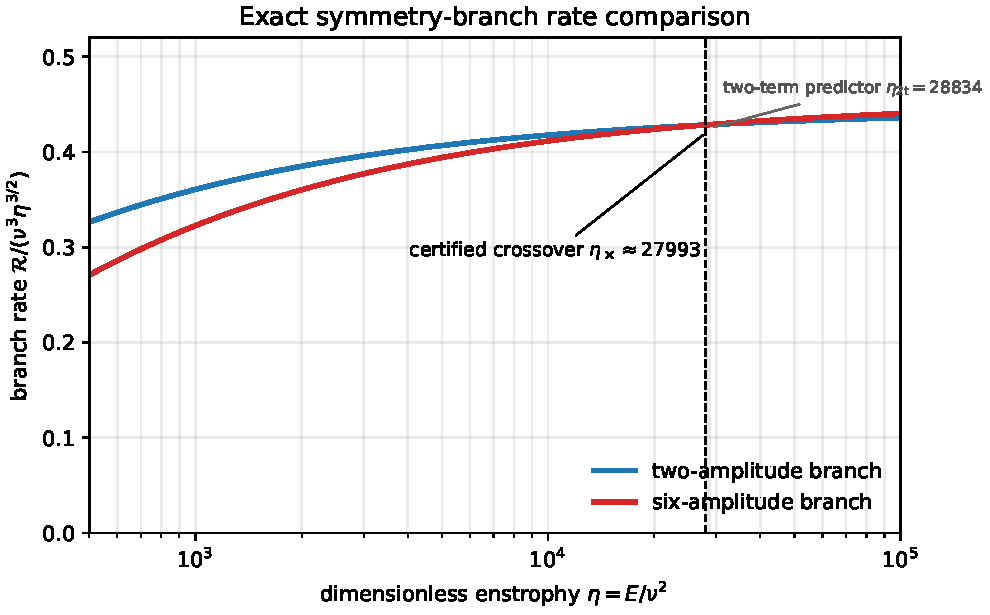
\includegraphics[width=0.82\linewidth]{figures/symmetry_branch_rates.pdf}
\caption{Exact reduced rate formulas for the two symmetry branches, normalized
by $\nu^3\eta^{3/2}$.  The vertical line marks the interval-certified crossover
from Theorem~\ref{thm:switch}; the adjacent gray sliver and annotation mark
the two-term asymptotic predictor, which is not used in that certification.
The plot compares only the two reduced branches; it is not an ordering of all
64-coordinate fields.}
\label{fig:branchrates}
\end{figure}

\begin{proof}[Proof certificate]
Eliminating $b$ from equality of rate and $\eta$ gives a degree-12 resultant
whose leading coefficient is positive and whose other coefficients are
negative.  It has exactly one positive root by Descartes' rule.  The map
$\eta(\mu)$ on the six-amplitude branch has positive derivative.  A
two-variable Krawczyk calculation encloses the crossing at both 256 and 512
bits; interval rate comparisons at $\eta=10^4$ and $4\times10^4$ establish
the two signs.  The machine-checkable polynomial and enclosures are archived
with the reproducibility artifacts listed below.
\end{proof}

\section{Conclusion}
The fixed-enstrophy instantaneous-production problem contains more exact
structure than is visible from numerical multistart optimization alone. In a
specified 16-pair Fourier class, we identify an ansatz-global six-amplitude
branch and a distinct exact two-amplitude full-KKT branch. At high parameter,
the latter is rigorously a higher full-space local maximum at a displayed
point, while the inviscid endpoint of the former is also a rigorously
certified full-space local maximum; moreover its entire high-$\eta$ branch is
uniformly locally maximal in the full Fourier class. At the inviscid endpoint the two branches
coexist as distinct full-space local maxima with an exact positive value gap.
Proposition~\ref{prop:shell112} adds an exact rational bound for one shellwise
component of stretching, rather than a global bound on the full cubic.
The two viscous branch rates undergo one certified switch. The result is a
finite-dimensional computer-assisted variational
theorem. Its main value is to expose and certify distinct mechanisms in a
standard extreme-flow problem, not to infer anything about arbitrary Fourier data
or long-time PDE dynamics.

\section{Reproducibility and scope}
The repository contains exact rational Fourier algebra, source hashes,
dependency manifests, and separate 256/512-bit Arb records.  Distinct
precisions protect against precision-specific numerical accidents, but they
are not a substitute for an independent implementation audit.  The command
\begin{verbatim}
python scripts/verify_paper_a.py
\end{verbatim}
recomputes the theorem claims, including the two-amplitude full-KKT branch and
the unique crossover.  The finite five-point sweep is retained as a
cross-check. The separate uniform certificate combines 188 rescaled low-$s$
intervals with 238 direct high-$s$ intervals and proves full-space local
maximality of the competing branch for every positive $\eta$; neither
certificate makes a full-space global claim.
An additional 2,048-box compact interval-continuation certificate proves the
same full-space local statement for the high-$\eta$ six-amplitude branch;
again it is a local finite-dimensional theorem only.
Proposition~\ref{prop:shell112} is independently exact: its rational Gram
identity verifies one shellwise cubic bound, but does not supply a global
bound on the full stretching term.

None of the results proves a full-space global maximum, extends beyond this
Fourier cutoff, or addresses a finite-time singularity or global regularity.

\paragraph{Artifact list.}
The content-addressed release manifest in the
{\ttfamily artifacts/proofs/} directory binds every checker, candidate,
source, manuscript file, and proof object by SHA-256. The primary proof
objects are:
\begin{center}
\begin{minipage}{0.94\linewidth}
\small\ttfamily
reduced\_static\_global\_arb\_certificate.json\\
reduced\_static\_standalone\_algebra\_audit.json\\
high\_branch\_eta10000\_arb\_certificate.json\\
inviscid\_six\_full64\_local\_certificate.json\\
inviscid\_competing\_full64\_local\_certificate.json\\
six\_branch\_high\_eta\_uniform.json\\
shell112\_sos\_certificate.json\\
shell123\_sos\_certificate.json\\
shell224\_sos\_certificate.json\\
shell334\_sos\_certificate.json\\
reduced\_competing\_formula.json\\
competing\_symmetry\_group.json\\
competing\_representation\_sectors.json\\
competing\_high\_eta\_uniform.json\\
competing\_all\_eta\_uniform.json\\
symmetry\_branch\_crossover.json
\end{minipage}
\end{center}
The one-command verifier is {\ttfamily scripts/verify\_paper\_a.py}. The
reviewer guide in the {\ttfamily paper/} directory gives the claim-to-artifact
map, including the exact symbolic spectral-continuation record and the
separate Arb interval records.

\bibliographystyle{plain}
\bibliography{references}
\end{document}
